\section{VALIDATION EVIDENCE, RECONSTRUCTABILITY, AND BENCHMARK READINESS}
\label{sec:validation_reproducibility}

Section~\ref{sec:metrics} showed that comparison depends on alignment across
the task, measurement plane, operating point, and validation setting. This
section examines how far those operating points were tested and how completely
their configurations can be reconstructed. It then relates validation settings,
evidence from both functions, and artifact access to benchmark readiness.

\subsection{Validation Settings and Methods}

Figure~\ref{fig:validation_profile} places each study's highest reported setting
beside the validation methods used across the corpus. The first panel assigns
one setting to every study, while the second allows several methods to
contribute to one evidence chain.

\begin{figure*}[!t]
\centering
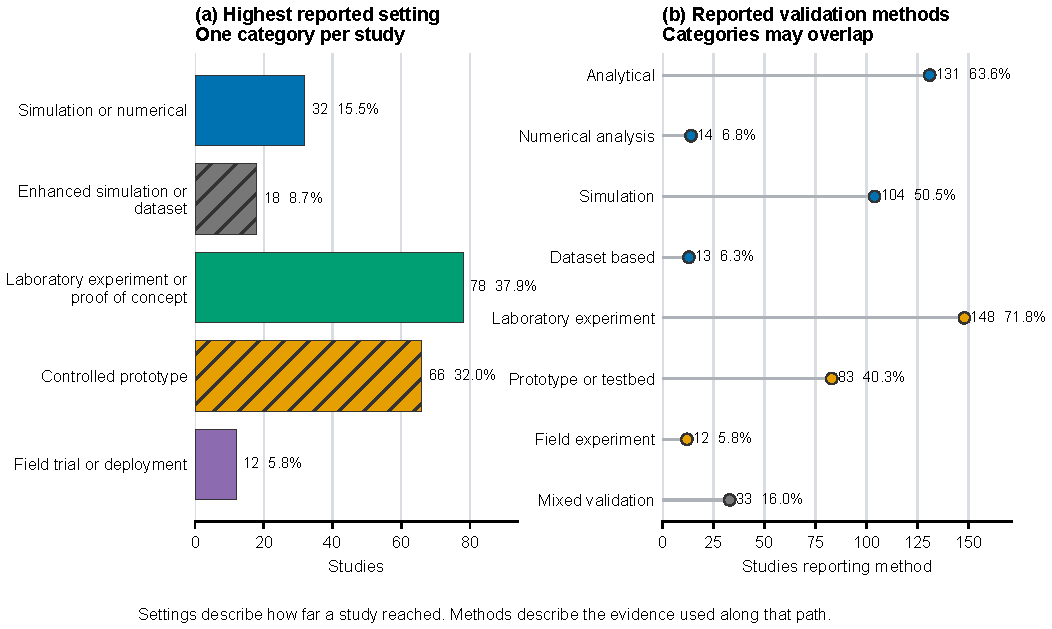
\includegraphics[width=\textwidth]{figures/final_submission_2026-08-25/fig07_validation_profile.pdf}
\caption{Validation settings and methods in the 206 studies. Panel (a) assigns
each study to one highest reported setting. Panel (b) reports analytical and
numerical methods, simulations, methods based on datasets, laboratory
experiments, prototypes, field studies, and mixed methods. Method categories may overlap because several
forms of evidence can contribute to one study. The panels describe the reach
and composition of validation as distinct properties.}
\label{fig:validation_profile}
\end{figure*}

The profile shows a broad laboratory and prototype base together with a smaller
field subset. Analytical, simulation, laboratory, and prototype methods can
contribute to one study, so the configuration trail across methods shapes
interpretation.

These settings expose different parts of an O-ISAC system. Simulation studies
isolate waveform and device sensitivities under controlled conditions
\cite{OISAC_SCR00007,OISAC_SCR00274}. Laboratory and prototype systems reveal
conversion, synchronization, and receiver effects in physical implementations
\cite{OISAC_SCR00001,OISAC_SCR00210,OISAC_SCR00362}. Field studies extend the
evidence to access networks, deployed fiber, submarine monitoring, and outdoor
wireless links
\cite{OISAC_SCR00496,OISAC_SCR00631,OISAC_SCR00957,OISAC_SCR01054,OISAC_SCR01086}.

The highest setting describes the reach of the evidence. Its scientific
meaning still depends on the claim and the test design. A controlled prototype
may explore a wider parameter range than a field trial, while a laboratory
experiment may reveal communication and sensing interactions more directly
than a field dataset collected for one outcome. The setting therefore gains
meaning when it is read together with the tested conditions, available
controls, and functional coverage.

Each method serves a different analytical purpose. Analysis clarifies
assumptions, simulation supports controlled parameter studies, and laboratory
work reveals the behavior of physical components. Prototypes bring subsystems
together, while field studies introduce at least one operational boundary.
Their combined value grows when the configuration and conditions remain
traceable as the evidence moves from one method to another.

Section~\ref{sec:optical_modality_families} shows that realistic validation
conditions change with the platform. Fiber studies depend on topology, traffic,
launch and receiver conditions, and the disturbance context. Visible light
communication and LiFi studies
add layout, orientation, illumination, detector, and processing conditions.
Free space optical studies require geometry, pointing, target properties,
weather, and motion. Terahertz systems enabled by photonics must also trace
optical conversion, antenna alignment, and wireless propagation. A useful
validation record therefore identifies the environment, measurement plane,
target or disturbance, reference method, and exercised function.

\subsection{Field Evidence Across Communication and Sensing}

The highest validation setting and the coverage of both functions answer
related questions. For 12 studies, a field trial or deployment was the
strongest reported setting. Six of them also received TQAF validation score 3
because their records report field or deployment outcomes in each functional
domain. The assessment is applied to each study. Electronic Supplement
S-Appraisal reports the corresponding scores. Electronic Supplement S7, the
paired function validation register, identifies the 12 studies and the subset
of six.

The six studies cover several settings. They include terahertz and cellular
links enabled by photonics, fiber access integrated with radio frequency
identification, and space laser ranging and communication. They also include
multicore fiber deployed in the field and submarine cable monitoring
\cite{OISAC_SCR01054,OISAC_SCR00496,OISAC_SCR00631,OISAC_SCR00730,OISAC_SCR01086,OISAC_SCR00957}.
Their diversity shows that field evidence for both functional domains appears
across several platforms. Platform comparisons still follow the native
validation conditions described in Section~\ref{sec:optical_modality_families}.

Electronic Supplement S7 records the available relationship timing and separate
source locators for the two functions. The six cases establish field or
deployment outcomes in both functional domains at the level of each study. Concurrent
joint operation is established when both outcomes are traceable to the same
configuration, time interval, and condition set.

The distinction becomes important when evidence is produced at different
stages of a system. One fiber study combines field data with offline sensing
classification and illustrates how field collection and functional execution
can occupy different parts of the evaluation path \cite{OISAC_SCR01006}.
Segmented architectures add interfaces, timing, calibration, and conversion
conditions to that path. When these elements connect both outcomes to one
operating point, field coverage can support a stronger claim of joint
operation.

\subsection{Artifact Access and Reconstructability}

Validation describes what a study tested. Reconstructability describes how
completely another group can recover the operating point and the path from
input to reported result. Access to data, code, or models supports this task,
while physical experiments also depend on the system configuration,
measurement conditions, processing steps, and provenance.

Table~\ref{tab:artifact_reconstruction} summarizes the access routes reported
for data and for code or models in all 206 studies.

\begin{table}[!t]
\caption{Reported access to data and to code or models in the 206 studies}
\label{tab:artifact_reconstruction}
\centering
\footnotesize
\setlength{\tabcolsep}{3.2pt}
\renewcommand{\arraystretch}{1.04}
\begin{tabularx}{\columnwidth}{@{}
>{\raggedright\arraybackslash}X
>{\centering\arraybackslash}p{0.28\columnwidth}@{}}
\toprule
Reported access & Studies, $n$ (\%) \\
\midrule
\multicolumn{2}{@{}l}{\textit{Data}} \\
Closed or status unreported & 145 (70.4\%) \\
Access by request & 41 (19.9\%) \\
Open access & 13 (6.3\%) \\
Outside artifact scope & 7 (3.4\%) \\
\addlinespace[2pt]
\multicolumn{2}{@{}l}{\textit{Code or model}} \\
Closed or status unreported & 197 (95.6\%) \\
Access by request & 7 (3.4\%) \\
Partial components & 1 (0.5\%) \\
Outside artifact scope & 1 (0.5\%) \\
\bottomrule
\end{tabularx}
\vspace{1pt}
\parbox{\columnwidth}{\raggedright\footnotesize\emph{Note.} The first row in
each group combines closed access and an unspecified access status.\par}
\end{table}

The reported routes support different forms of reconstruction. Open data
appear across simulation, laboratory, prototype, computer vision, and field
data settings
\cite{OISAC_SCR00274,OISAC_SCR00362,OISAC_SCR00833,OISAC_SCR01006,OISAC_SCR01008}.
They support reanalysis of the released data. Complete system reconstruction
also requires configuration and execution details. Software preserves the
transformation from inputs to reported outputs, and one computer vision study
reported partial code or model components
\cite{OISAC_SCR00833}.

Reconstructing a physical experiment requires the system and hardware, the
scene and calibration, the waveform and processing, the metrics and data, and
the versioned release. These requirements extend the comparison profile in
Section~\ref{sec:foundations_comparison}. Electronic Supplements S-Data
Dictionary and S-Evidence provide the field definitions and record provenance
used in the review.

The TQAF reproducibility assessment reads artifact access together with
parameter reporting. It places 4 studies in the low category, 199 in the
adequate category, and 3 in the strong category. Electronic Supplement
S-Appraisal provides scores for each study. Thirteen studies report open data,
while three reach strong reproducibility. The difference reflects the
additional reconstruction information captured by the appraisal.

\subsection{Benchmark Readiness}

A reconstructable result becomes a reusable benchmark when another group can
apply the same task, condition set, baseline, and metric definition. The TQAF
benchmark assessment combines these requirements with artifact access,
validation, reproducibility, and comparison admissibility. The observed
distribution comprises 48 studies in the low category, 158 in the adequate
category, and zero in the strong category.

Under the review criteria, strong readiness depends on bringing an external or
common baseline, an open artifact, admissible outcomes in both functional
domains, and strong validation and reproducibility support into the same
evidence chain. S-Appraisal reports these scores. This distribution directs
attention toward shared tasks, baselines,
artifacts, and evaluation conditions that other groups can reuse.

These distributions characterize evidence reach, functional coverage, artifact
access, and reconstructability within the 206 included studies. They provide
the descriptive basis for the benchmark and reporting actions in
Section~\ref{sec:discussion_roadmap}.

Overall, the corpus combines a broad laboratory and prototype base with a
smaller set of field and deployment results. Stronger cumulative evidence
emerges when both functions are tied to one traceable configuration and the
evaluation path is preserved through reusable artifacts. Section~\ref{sec:technologies_applications_6g}
builds on this validation map by examining the technologies and applications
supported by the reported evidence and their connection to 6G network roles.
